\section{Results}\label{sec:results}
We evaluated \tool using both real and simulated sequencing datasets (Supplementary Section~\ref{supsec:datasets}).
For comparison, we ran competing PacBio HiFi-based callers using minimap2 alignments generated from identical read sets (Supplementary Section~\ref{supsec:tools}) and constructed consensus truth sets using Minda~\cite{minda} (Supplementary Section~\ref{supsec:consensus}).
Supplementary Sections~\ref{supsec:simgen} and~\ref{supsec:simeval} detail the simulated dataset generation and truth-set construction.
To assess significance, we computed 95\% bootstrap confidence intervals for the F1 score differences between \tool and the best other caller across 2,000 resamples (sampling consensus SVs with replacement for recall and candidate calls for precision).
We calculated two-sided uncorrected $p$-values as twice the smaller tail probability relative to zero. 

End-to-end analysis using \tool starting from reads completed in $\sim$13 minutes per tumor-normal pair. We report full benchmarks of the computational requirements of \tool in Supplementary Section~\ref{supsec:compute}.

%%%%%%%%% CAN HERE.  
\subsection{Accuracy on real tumor--normal pairs}\label{sec:accuracy}

We first evaluated \tool{} using five tumor--normal cell line pairs from the CASTLE panel with PacBio HiFi data~\cite{severus} with normal samples at 41--71$\times$ and tumor samples at 58--65$\times$ (Table~\ref{tab:castle}).

\junk{Since no curated set of somatic SVs exists for these cell lines, the panel provides a consensus generated by Minda~\cite{minda} from 11 call sets, retaining calls found with at least two of the three technologies and in at least four call sets.
The 11 call sets come from Severus~\cite{severus}, SAVANA~\cite{savana}, nanomonsv~\cite{nanomonsv}, and Sniffles2~\cite{sniffles2} on both PacBio HiFi and ONT data, and from SvABA~\cite{svaba}, GRIPSS~\cite{gripss}, and Manta~\cite{manta} on Illumina data.
Because this consensus includes only four of the 10 callers that we ran on the PacBio HiFi reads, we rebuilt it from 18 call sets, namely \tool{}, our own runs of these 10 callers (Severus, SAVANA, nanomonsv, Sniffles2, dysgu~\cite{dysgu}, SVision-pro~\cite{svisionpro}, cuteSV~\cite{cutesv}, DeBreak~\cite{debreak}, kled~\cite{kled}, and SVDSS~\cite{svdss}; Supplementary Section~\ref{supsec:tools}), and the seven ONT and Illumina call sets of the panel.
We kept the requirement of support by at least two technologies but raised the minimum number of supporting call sets to six (Supplementary Section~\ref{supsec:consensus}).
In this consensus, every call set we compare, including \tool{}, contributes to the truth set under the same criteria.
In all comparisons, we ran Minda with a breakpoint tolerance of 500\,bp and a minimum SV length of 50\,bp.
}

Due to the lack of a curated somatic SV ground truth for these cell lines, the CASTLE panel provides an 11-call-set consensus generated by Minda~\cite{minda}, requiring support by at least two technologies and four callers across PacBio HiFi, ONT, and Illumina platforms~\cite{severus,savana,nanomonsv,sniffles2,svaba,gripss,manta}. Because that consensus encompasses only four of the ten PacBio callers evaluated here, we expanded the truth set to 18 call sets by incorporating \tool{}, our runs of all ten PacBio callers (Severus, SAVANA, nanomonsv, Sniffles2, dysgu~\cite{dysgu}, SVision-pro~\cite{svisionpro}, cuteSV~\cite{cutesv}, DeBreak~\cite{debreak}, kled~\cite{kled}, and SVDSS~\cite{svdss}; Supplementary Section~\ref{supsec:tools}), and the panel's seven ONT and Illumina call sets. To ensure unbiased benchmarking, we maintained the two-technology requirement, raised the caller threshold to six, and applied uniform Minda parameters (500\,bp breakpoint tolerance, 50\,bp minimum size) across all evaluations (Supplementary Section~\ref{supsec:consensus}).

We classified each pair with a model trained on the other four (leave-one-out cross-validation; Methods).
Against the consensus of 18 call sets, the F1 score then ranged from 0.850 for NCI-H1437 to 0.928 for NCI-H2009 (Table~\ref{tab:castle}).
Precision was lowest for HCC1937, and recall was lowest for NCI-H1437, whose consensus contains only 222 SVs.
Supplementary Section~\ref{supsec:missed} analyzes the consensus SVs that \tool{} did not call.
The training labels come from the published consensus of 11 call sets (Methods), with the seven ONT and Illumina call sets also included in the evaluation consensus.
A model trained instead with labels from the 17 call sets other than \tool{} reached a mean F1 score of 0.887 instead of 0.881 (Supplementary Section~\ref{supsec:classifier}).

\begin{table}[tbp]
\centering
\caption{Accuracy of \tool{} on the five CASTLE pairs}
\label{tab:castle}
\begin{tabular}{lrrrrrrrrr}
\toprule
Pair & Coverage & Truth & Calls & TP & FP & FN & Precision & Recall & F1 \\
     & n/t      &       &       &    &    &    &           &        &    \\
\midrule
HCC1954   & 62.9/63.3 & 1,059 & 1,134 &  997 & 137 &  62 & 0.879 & 0.941 & 0.909 \\
NCI-H2009 & 68.1/65.1 &  899 &  925 &  846 &  79 &  53 & 0.915 & 0.941 & 0.928 \\
HCC1937   & 56.0/59.8 &  697 &  701 &  602 &  99 &  95 & 0.859 & 0.864 & 0.861 \\
NCI-H1437 & 71.1/64.5 &  222 &  206 &  182 &  24 &  40 & 0.883 & 0.820 & 0.850 \\
HCC1395   & 41.3/58.3 & 1,284 & 1,248 & 1,082 & 166 & 202 & 0.867 & 0.843 & 0.855 \\
\bottomrule
\end{tabular}
\tabnotes{Precision, recall, and F1 score of \tool{} against the consensus of 18 call sets.
A model trained on the other four pairs classifies each pair. n/t, normal/tumor; TP, true positives; FP, false positives; FN, false negatives.}
\end{table}

\begin{figure}[tbp]
\centering
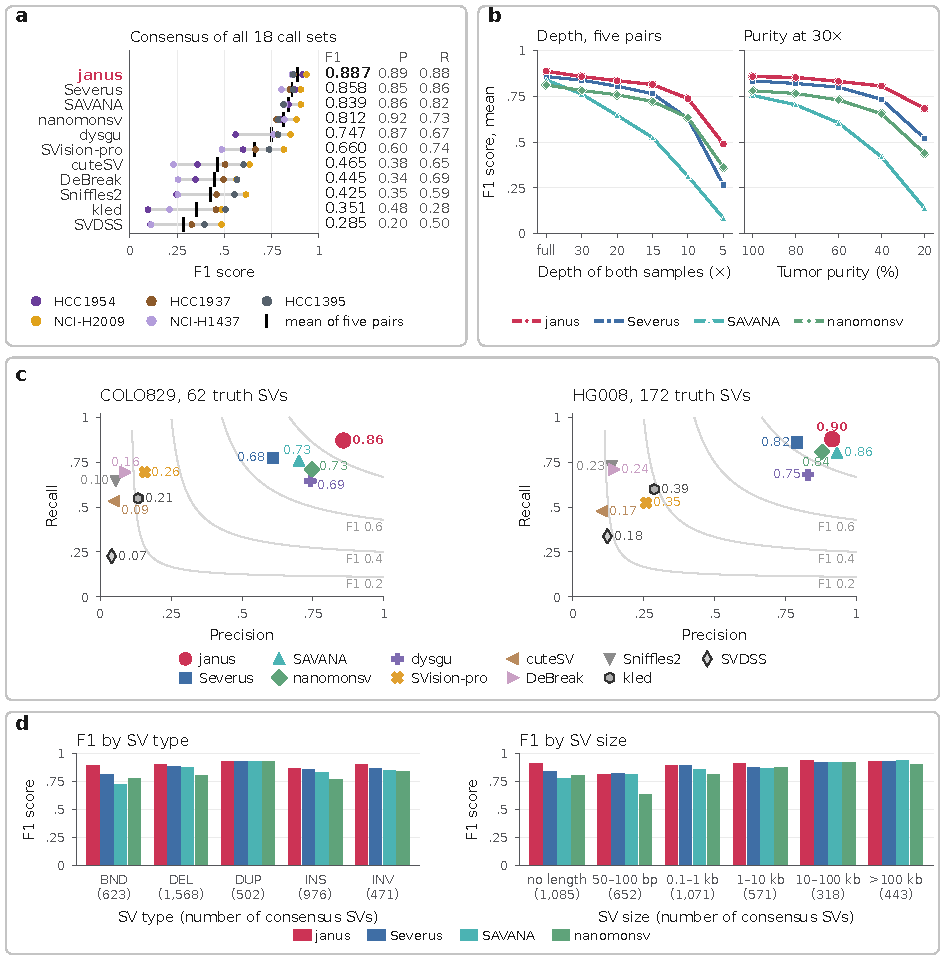
\includegraphics[width=157mm]{figures/fig_accuracy.pdf}
\caption{Accuracy of \tool{} and the other callers. (a) F1 score of the 11 PacBio HiFi call sets per CASTLE pair (dots) and the mean over pairs (bar), against the consensus of all 18 call sets and of the 17 other than \tool{} (P, precision; R, recall). (b, c) Precision and recall on COLO829 (b) and HG008 (c), with curves of equal F1 score and the bootstrap 95\% interval of the F1 difference from the best other caller. (d, e) F1 score by SV type (d) and size (e), five pairs pooled; inversions include inverted junctions; first size class: SVs without length; consensus SVs in parentheses. (f--i) F1 score (f, h) and precision and recall (g, i) at reduced depth (f, g) and purity (h, i).
Shading: bootstrap 95\% interval of \tool{}; above (f, h): bootstrap $p$-value against the best other caller, red if $p<0.05$.}
\label{fig:castle}
\end{figure}

Against the consensus of all 18 call sets, \tool{} had the highest mean F1 score (0.881; Figure~\ref{fig:castle}a, Supplementary Figure~\ref{supfig:allsets}), ahead of Severus (0.858 on PacBio HiFi and 0.843 on ONT data) and of the PacBio HiFi call sets of SAVANA (0.837) and nanomonsv (0.810).
It ranked first in four of the five pairs, the exception being HCC1395, where both Severus call sets scored higher (Figure~\ref{fig:castle}a, Supplementary Figure~\ref{supfig:allsets}).
For SAVANA and nanomonsv, the ONT call sets had lower F1 scores and lower precision than the PacBio HiFi call sets (Supplementary Figure~\ref{supfig:allsets}).
Of the Illumina call sets, Manta (mean F1 score 0.600) and GRIPSS (0.565) scored above Sniffles2 on ONT data (0.489) and above five PacBio HiFi call sets, and SvABA (0.403) scored above kled and SVDSS only; all three varied widely between pairs.
As the Severus study reported for the original consensus~\cite{severus}, all three performed best in HCC1954 and worst in NCI-H2009 (Supplementary Table~\ref{suptab:allwith}).
nanomonsv on PacBio HiFi data had the highest precision of all call sets, but its recall was lower than that of \tool{}, Severus, and SAVANA (Supplementary Figure~\ref{supfig:allsets}).
Among the PacBio HiFi call sets, \tool{} had the highest recall.

We also scored all call sets against the consensus of the 17 call sets other than \tool{}, in which every caller except \tool{} still contributes to its own truth set.
Severus on PacBio HiFi data then had the highest mean F1 score (0.859), followed by \tool{} (0.857) and SAVANA (0.847; Figure~\ref{fig:castle}a).
Following the Severus study~\cite{severus}, we finally scored each of the 11 PacBio HiFi call sets against the consensus of the 17 others, so that no call set contributes to its own truth set (for \tool{}, this is the consensus without \tool{} above; Supplementary Section~\ref{supsec:loo}, Supplementary Figure~\ref{supfig:allsets}c).
In this comparison, \tool{} ranked first in all five pairs with a mean F1 score of 0.857, compared with 0.832 for Severus and 0.823 for SAVANA.

We also tested two pairs outside the training data whose truth sets are independent of our calls.
COLO829 is a melanoma cell line with 68 somatic SVs validated with several technologies~\cite{colo829}, of which 62 are at least 50\,bp long.
For HG008, a pancreatic tumor with a matched normal sample, the Genome in a Bottle Consortium released a draft somatic SV benchmark (v0.5)~\cite{hg008}.
We classified both pairs with the model trained on all five CASTLE pairs.
We ran the other PacBio HiFi callers with the same parameters as for CASTLE and scored all call sets with Minda as above (Supplementary Section~\ref{supsec:consensus}).
On both pairs, \tool{} reached the highest F1 score and recall of the PacBio HiFi callers (Table~\ref{tab:external}, Figure~\ref{fig:castle}b,c).
On COLO829, its 65 calls matched 54 SVs (F1 score 0.850), compared with 0.729 for SAVANA, 0.727 for nanomonsv, 0.690 for dysgu, and 0.681 for Severus, and the difference from SAVANA was 0.122 (bootstrap 95\% interval 0.020 to 0.226).
On HG008, its F1 score was 0.886, compared with 0.863 for SAVANA, 0.842 for nanomonsv, and 0.825 for Severus, and the difference from SAVANA was 0.023 (bootstrap 95\% interval $-$0.030 to 0.077).
The two truth sets contain 62 and 172 SVs of at least 50\,bp, compared with 4,161 consensus SVs in the five CASTLE pairs together.

When we pooled the five pairs, \tool{} had a higher F1 score than the four PacBio HiFi callers of the published consensus for breakends, deletions, insertions, inversions, and SVs of 1--100\,kb.
For duplications, SAVANA, Severus, and nanomonsv scored higher than \tool{}, and for SVs larger than 100\,kb, SAVANA and Severus did; Severus also scored higher for SVs of 0.1--1\,kb, as did Severus and SAVANA for SVs of 50--100\,bp (Figure~\ref{fig:castle}d,e; Supplementary Table~\ref{suptab:types}).

\begin{table}[tbp]
\centering
\caption{PacBio HiFi callers on COLO829 and HG008}
\label{tab:external}
\small
\resizebox{\ifdim\width>\textwidth\textwidth\else\width\fi}{!}{\begin{tabular}{lrrrrrrrr}
\toprule
 & \multicolumn{4}{c}{COLO829} & \multicolumn{4}{c}{HG008} \\
Caller & Calls & Precision & Recall & F1 & Calls & Precision & Recall & F1 \\
\midrule
\tool{} & 65 & 0.831 & 0.871 & \textbf{0.850} & 169 & 0.893 & 0.878 & \textbf{0.886} \\
SAVANA & 67 & 0.701 & 0.758 & 0.729 & 148 & 0.932 & 0.802 & 0.863 \\
nanomonsv & 59 & 0.746 & 0.710 & 0.727 & 158 & 0.880 & 0.808 & 0.842 \\
dysgu & 54 & 0.741 & 0.645 & 0.690 & 141 & 0.830 & 0.680 & 0.748 \\
Severus & 79 & 0.608 & 0.774 & 0.681 & 187 & 0.791 & 0.860 & 0.825 \\
SVision-pro & 275 & 0.156 & 0.694 & 0.255 & 348 & 0.259 & 0.523 & 0.346 \\
kled & 256 & 0.133 & 0.548 & 0.214 & 359 & 0.287 & 0.599 & 0.388 \\
DeBreak & 491 & 0.088 & 0.694 & 0.156 & 843 & 0.145 & 0.709 & 0.240 \\
Sniffles2 & 743 & 0.054 & 0.645 & 0.099 & 912 & 0.137 & 0.727 & 0.231 \\
cuteSV & 689 & 0.048 & 0.532 & 0.088 & 794 & 0.103 & 0.477 & 0.170 \\
SVDSS & 352 & 0.040 & 0.226 & 0.068 & 476 & 0.122 & 0.337 & 0.179 \\
\bottomrule
\end{tabular}}
\tabnotes{PacBio HiFi callers on COLO829 (62 validated somatic SVs of at least 50\,bp) and HG008 (draft benchmark v0.5), scored with Minda; neither pair was part of the training data.
Rows ordered by F1 score on COLO829; bold: highest.}
\end{table}

We downsampled both read sets of the five CASTLE pairs to 30$\times$, 20$\times$, 15$\times$, 10$\times$, and 5$\times$.
For lower tumor purity, we mixed tumor reads with reads of the matched normal sample that we had left out of the normal read set of the run, producing 30$\times$ read sets of 100\% to 20\% tumor purity.
We ran Severus, SAVANA, and nanomonsv, the three other PacBio HiFi callers with the highest mean F1 scores (Table~\ref{tab:callers}), on the same downsampled read sets and on the purity mixtures of all five pairs.
We classified all read sets of a pair with the same model and scored them against the consensus of the full-depth pair (Figure~\ref{fig:castle}f--i; Supplementary Section~\ref{supsec:depth}).
Between 30$\times$ and 5$\times$, the mean F1 score of \tool{} decreased from 0.856 to 0.476, mainly because recall fell from 0.863 to 0.387.
The F1 score of Severus fell more steeply than that of \tool{} over the same range, from 0.838 to 0.264, as its recall dropped to 0.164.
At 20\% purity, \tool{} reached a mean precision of 0.870 and a mean F1 score of 0.679 over the five pairs, compared with a mean F1 score of 0.520 for Severus.

\begin{table}[tbp]
\centering
\caption{F1 score of the PacBio HiFi callers on the five CASTLE pairs}
\label{tab:callers}
\small
\setlength{\tabcolsep}{4pt}
\resizebox{\textwidth}{!}{%
\begin{tabular}{lrrrrrrrrrrrrr}
\toprule
 & \multicolumn{6}{c}{Consensus of 18 call sets} & \multicolumn{6}{c}{Consensus of 17 call sets, without \tool{}} & \\
\cmidrule(lr){2-7}\cmidrule(lr){8-13}
Caller & HCC1954 & NCI-H2009 & HCC1937 & NCI-H1437 & HCC1395 & Mean & HCC1954 & NCI-H2009 & HCC1937 & NCI-H1437 & HCC1395 & Mean & Time (h:mm) \\
\midrule
\tool{}     & \textbf{0.909} & \textbf{0.928} & \textbf{0.861} & \textbf{0.850} & 0.855 & \textbf{0.881} & 0.869 & \textbf{0.914} & 0.829 & \textbf{0.831} & 0.842 & 0.857 & 0:11 \\
Severus     & 0.873 & 0.905 & 0.846 & 0.799 & \textbf{0.866} & 0.858 & \textbf{0.886} & 0.904 & \textbf{0.848} & 0.798 & \textbf{0.861} & \textbf{0.859} & 6:24 \\
SAVANA      & 0.835 & 0.903 & 0.817 & 0.818 & 0.813 & 0.837 & 0.860 & 0.904 & 0.827 & 0.827 & 0.818 & 0.847 & 5:39 \\
nanomonsv   & 0.795 & 0.880 & 0.774 & 0.816 & 0.784 & 0.810 & 0.824 & 0.881 & 0.783 & 0.830 & 0.787 & 0.821 & 5:27 \\
dysgu       & 0.557 & 0.848 & 0.781 & 0.753 & 0.784 & 0.745 & 0.583 & 0.851 & 0.790 & 0.762 & 0.786 & 0.754 & 4:23 \\
SVision-pro & 0.597 & 0.815 & 0.664 & 0.486 & 0.739 & 0.660 & 0.608 & 0.817 & 0.664 & 0.485 & 0.738 & 0.662 & 4:44 \\
cuteSV      & 0.356 & 0.632 & 0.503 & 0.229 & 0.601 & 0.464 & 0.355 & 0.632 & 0.509 & 0.230 & 0.605 & 0.466 & 4:21 \\
DeBreak     & 0.346 & 0.563 & 0.495 & 0.253 & 0.566 & 0.445 & 0.355 & 0.564 & 0.497 & 0.254 & 0.569 & 0.448 & 4:25 \\
Sniffles2   & 0.245 & 0.613 & 0.459 & 0.251 & 0.553 & 0.424 & 0.254 & 0.615 & 0.463 & 0.253 & 0.555 & 0.428 & 4:22 \\
kled        & 0.095 & 0.485 & 0.455 & 0.210 & 0.504 & 0.350 & 0.099 & 0.489 & 0.464 & 0.213 & 0.510 & 0.355 & 4:21 \\
SVDSS       & 0.107 & 0.484 & 0.328 & 0.110 & 0.394 & 0.284 & 0.108 & 0.483 & 0.323 & 0.109 & 0.394 & 0.284 & 6:36 \\
\bottomrule
\end{tabular}}
\tabnotes{F1 score of \tool{} and of the callers we ran on the same PacBio HiFi reads, against the consensus of all 18 call sets and of the 17 call sets other than \tool{} (bold: highest).
Time: wall clock on HCC1954 from the read sets to the calls on 16 threads (SAVANA on 8), including mapping (4:19) and, for Severus and SAVANA, phasing.}
\end{table}

\junk{
\subsection{Runtime and memory per pair}

All tools ran on a workstation with an AMD Ryzen 9 9950X CPU (16 cores) and 196\,GB of memory, using 16 threads (8 for SAVANA, because SAVANA with 16 threads exceeded the available memory). Memory values are peak resident set sizes (RSS); memory and file sizes are given in GB.

Starting from the FASTQ files, \tool{} took 8 min to 13 min 12 s per pair (Table~\ref{suptab:time}, Figure~\ref{supfig:cost}a). Most of this time, 4.7--7.9 min, went into packing the reads and extracting the cores. Building the graph and detecting the sites took less than 2 min, and selecting, placing, and aligning the snippets took 1--4 min. The peak memory of 10.8--12.2\,GB was reached by minimap2 when aligning the snippets or their unaligned parts, whereas the steps of \tool{} itself used up to 9.7\,GB (Figure~\ref{supfig:cost}b). Training one classifier model took 4--25 seconds, and the complete classification step for all 77 runs on real data (the full-depth, downsampled, and mixed read sets of the seven pairs), including the threshold selection, took 3.8 minutes.

\begin{table}[tbp]
\centering
\small
\begin{tabular}{lrrrrrr}
\toprule
Stage & HCC1954 & NCI-H2009 & HCC1937 & NCI-H1437 & HCC1395 & Peak RSS (GB) \\
\midrule
Packing           & 3:55 & 4:44 & 4:06 & 3:56 & 2:20 & 4.4--9.0 \\
Core extraction   & 2:58 & 3:09 & 2:44 & 3:12 & 2:21 & 0.2 \\
Counting          & 0:53 & 0:51 & 0:49 & 0:54 & 0:38 & 6.6--7.4 \\
Graph and pruning & 0:53 & 0:55 & 0:48 & 0:51 & 0:43 & 8.7--9.7 \\
Selection         & 0:22 & 0:22 & 0:19 & 0:20 & 0:19 & 5.5--5.7 \\
Placement         & 0:06 & 0:06 & 0:04 & 0:04 & 0:05 & 4.2--5.0 \\
minimap2          & 3:19 & 2:31 & 0:41 & 1:29 & 1:10 & 10.8--12.2 \\
Calling           & 0:30 & 0:33 & 0:26 & 0:30 & 0:24 & 5.0--5.2 \\
\midrule
Total             & 12:55 & 13:12 & 9:56 & 11:17 & 8:00 & 10.8--12.2 \\
\bottomrule
\end{tabular}
\caption{Wall-clock time (m:ss) per stage on 16 threads and range of peak resident memory over the five pairs.}
\label{suptab:time}
\end{table}

On disk, the intermediate files of \tool{} require 90--121\,GB per pair, most of this space for the packed reads, whereas the two sorted BAM files needed by the alignment-based callers require 117--167\,GB, which is on average 38\% more (Figure~\ref{supfig:cost}c, Table~\ref{suptab:mapping}; details in Supplementary Section~\ref{supsec:files}).

Mapping both read sets of HCC1954 with minimap2 and sorting the alignments took 4 h 19 min with a peak memory of 19.3\,GB, and the complete \tool{} run on this pair needed about 5\% of this time (Table~\ref{suptab:mapping}) and 63\% of this memory (12.2\,GB); for the other four pairs, we estimated the mapping time at 3.5--4.8 hours. With variant calling included, the alignment-based pipelines took from 4 h 21 min (cuteSV and kled) to 6 h 36 min (SVDSS) on HCC1954, and Severus (6 h 24 min) and SAVANA (5 h 39 min) each spent 56 minutes of their run time on phasing with Clair3~\cite{clair3} and LongPhase~\cite{longphase} (Table~\ref{tab:callers}, Figure~\ref{supfig:cost}d).

The snippets that \tool{} aligned amounted to 0.34--1.12\,Gbp per pair, which is 0.09--0.29\% of the 309--420\,Gbp of the two read sets of the same pair (Figure~\ref{supfig:cost}e, Table~\ref{suptab:mapping}). No read of the normal sample was aligned. In CPU time, \tool{} used 2.3 hours on HCC1954, whereas mapping alone used 55 hours and the complete pipelines of the other callers 55--81 hours (Figure~\ref{supfig:cost}f). From 11.6--12.7 million tumor reads per pair, \tool{} detected 90,000--304,000 sites, cut 26,000--89,000 snippets, and wrote 2,300--5,300 records (Figure~\ref{supfig:cost}g, Supplementary Table~\ref{suptab:steps}).

\begin{table}[tbp]
\centering
\begin{tabular}{lrrrrr}
\toprule
Pair & Reads (Gbp) & Mapping (h:mm) & \tool{} (m:ss) & Ratio & Alignments (GB) \\
\midrule
HCC1954   & 391 & 4:19 & 12:55 & 20.0 & 165 \\
NCI-H2009 & 413 & 4:44$^\dagger$ & 13:12 & 21.5$^\dagger$ & 167 \\
HCC1937   & 359 & 4:07$^\dagger$ & 9:56 & 24.8$^\dagger$ & 144 \\
NCI-H1437 & 420 & 4:49$^\dagger$ & 11:17 & 25.6$^\dagger$ & 167 \\
HCC1395   & 309 & 3:32$^\dagger$ & 8:00 & 26.5$^\dagger$ & 117 \\
\bottomrule
\end{tabular}
\caption{Mapping the two read sets of a pair with minimap2 on 16 threads and size of the alignment files, compared with the complete run of \tool{}. $^\dagger$Estimated from the amount of sequence at the mean throughput of HCC1954 and COLO829 (39.6 and 42.8\,s per Gbp).}
\label{suptab:mapping}
\end{table}

\begin{figure}[tbp]
\centering
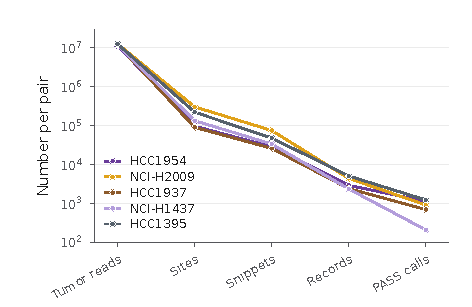
\includegraphics[width=\textwidth]{figures/fig_cost.pdf}
\caption{Cost of \tool{} and of the alignment-based pipelines on 16 threads (SAVANA on 8 threads). (a) Wall-clock time of \tool{} by stage. (b) Resident memory over a run: median (line) and range (band) of the five pairs; dashed: peak of minimap2 mapping HCC1954. (c) Disk use, mean of the five pairs. (d) Wall-clock time from the read sets to the calls on HCC1954, with the factor relative to \tool{}. (e) Sequence aligned per pair: both read sets for minimap2, snippets for \tool{}. (f) CPU time on HCC1954. (g) Tumor reads, sites, snippets, records, and PASS calls per pair.}
\label{supfig:cost}
\end{figure}

}

\subsection{Calling SVs in multiple tumors within one personal pangenome}\label{sec:multiple}

As no public long-read dataset has many tumor samples from one patient and a known set of somatic SVs, we evaluated joint calling on simulated data: one normal genome with the germline variants of a real individual, and 20 tumor genomes related by a tree, each inheriting the somatic variants of its ancestors (Supplementary Section~\ref{supsec:simgen}).
The simulation contains 5,147 SVs, and each tumor carries 1,016--1,353 SVs of at least 50\,bp.
We simulated PacBio HiFi reads at 20$\times$ per genome and downsampled them to 10$\times$ and 5$\times$, giving five normal/tumor depths (Table~\ref{tab:sim}).
At 20/20, all samples have the same moderate depth; at 10/10 and 5/5, all samples have low depth.
20/10 and 20/5 correspond to a normal sample sequenced once at moderate depth and to a tumor sequencing budget divided among many samples; low tumor depth can also be unavoidable when a sample yields little DNA, for example, in designs that approach single-cell resolution. 

We matched calls to the junctions that each simulated SV creates, with a 500\,bp tolerance and a 50\,bp minimum SV length; an SV with several junctions, such as a translocation or a dispersed duplication, therefore counts as detected if a call matches at least one of its junctions (Supplementary Section~\ref{supsec:simeval}).
The truth set of each tumor retains 9--13\% of its SVs that arose on a chromosome copy later lost in an ancestor of the tumor, even though no reads support them.

\begin{figure}[tbp]
\centering
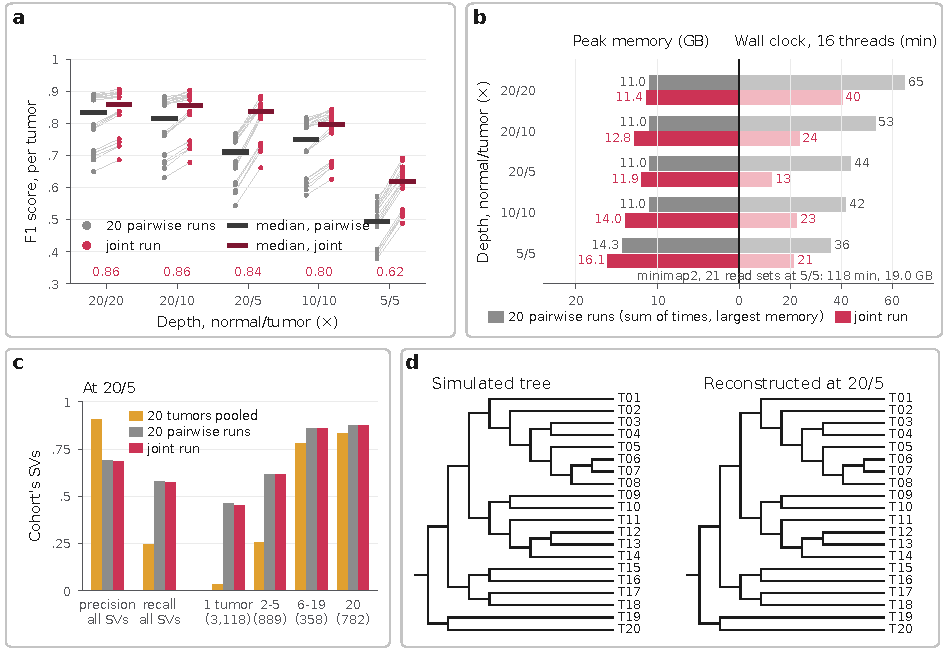
\includegraphics[width=\textwidth]{figures/fig_sim.pdf}
\caption{A simulated case with one normal and 20 tumors at five normal/tumor depths. (a) The simulated tree and the tree reconstructed from the joint calls at 20/5. (b) Share of called SVs whose tumors form one clade, with the number of the 17 splits recovered. (c--e) Precision, recall, and F1 score per tumor for the pairwise and joint runs; bars: medians over the 20 tumors. (f) Wall-clock time from the packed reads; dashed: minimap2 on the 21 read sets at 5/5. (g) Peak memory; dashed: minimap2 at 5/5.}
\label{fig:sim}
\end{figure}

\begin{table}[tbp]
\centering
\caption{Pairwise and joint runs on the simulated case}
\label{tab:sim}
\small
\resizebox{\textwidth}{!}{%
\begin{tabular}{lrrrrrrrrrrrr}
\toprule
 & \multicolumn{3}{c}{Pairwise runs} & \multicolumn{3}{c}{Joint run} & \multicolumn{2}{c}{Tree} & \multicolumn{2}{c}{Wall clock (min)} & \multicolumn{2}{c}{Peak RSS (GB)} \\
Coverage n/t & Precision & Recall & F1 & Precision & Recall & F1 & Splits & RF & Pairwise & Joint & Pairwise & Joint \\
\midrule
20/20 & 0.894 & 0.782 & 0.834 & 0.914 & 0.803 & 0.856 & 17/17 & 0 & 64.9 & 40.4 & 11.0 & 11.4 \\
20/10 & 0.890 & 0.751 & 0.815 & 0.894 & 0.786 & 0.838 & 17/17 & 0 & 53.4 & 23.5 & 11.0 & 12.8 \\
20/5  & 0.904 & 0.586 & 0.711 & 0.914 & 0.701 & 0.794 & 16/17 & 2 & 43.7 & 12.8 & 11.0 & 11.9 \\
10/10 & 0.799 & 0.715 & 0.755 & 0.819 & 0.761 & 0.789 & 17/17 & 0 & 41.8 & 22.6 & 11.0 & 14.0 \\
5/5   & 0.483 & 0.512 & 0.498 & 0.544 & 0.636 & 0.586 & 17/17 & 0 & 35.9 & 21.5 & 14.3 & 16.1 \\
\bottomrule
\end{tabular}}
\tabnotes{The simulated case at five normal/tumor depths.
Precision, recall, and F1 score: medians over the 20 tumors.
Splits: splits of the simulated tree found in the reconstructed tree; RF: Robinson--Foulds distance.
Wall-clock time and peak memory on 16 threads from the packed reads (pairwise: sum of the times, largest memory).
minimap2 mapped the 21 read sets at 5/5 in 117.6 min with 19.0\,GB.
RSS, resident set size.}
\end{table}

We called each tumor in two ways: separately against the normal sample (20 pairwise runs), and together with all other samples in a single graph of the 21 read sets (joint run).
At 20/5, the joint run raised the median F1 score from 0.711 to 0.794 and scored higher for each of the 20 tumors (Table~\ref{tab:sim}, Figure~\ref{fig:sim}c--e).
The gain came mostly from recall, which increased from 0.586 to 0.701, and precision rose from 0.904 to 0.914.
The joint run had the higher median F1 score at all five depths, although the margin was smaller at higher tumor depth (0.856 compared with 0.834 at 20/20).
Part of this gain comes from the classification step, in which \tool{} accepts a record of the joint run at a lower probability if another tumor has a record of the same SV that reaches its own threshold, and at a higher probability otherwise (Methods).

Starting from the packed reads, the joint run called the 20 tumors in 12.8 min, 3.4 times faster than the 20 pairwise runs together (43.7 min; Figure~\ref{fig:sim}f).
Its memory, however, exceeded that of the largest pairwise run at all five depths (11.9 compared with 11.0\,GB at 20/5; Figure~\ref{fig:sim}g).
Mapping and sorting the 21 read sets with minimap2, without any variant calling, took 1 h 58 min at 5/5 and, by extrapolation, about 7.7 h at 20/20.

Finally, we reconstructed the tree of the 20 tumors from the joint calls.
After we merged records of the same SV across different tumors, the joint run at 20/5 contained 6,123 SVs, including 2,047 false calls, 1,922 of them called in only one tumor.
For 4,822 of the 6,123 SVs (79\%), the set of carrier tumors was exactly one clade of the simulated tree, a single tumor counting as a clade (Figure~\ref{fig:sim}b).
We then built a neighbor-joining tree in which the distance between two tumors is the number of SVs called in only one of them.
This tree recovered 16 of the 17 splits of the simulated tree (Robinson--Foulds distance 2; Figure~\ref{fig:sim}a, drawn with the simulated root).
The trees at 20/20, 20/10, 10/10, and 5/5 had the unrooted topology of the simulated tree (Table~\ref{tab:sim}).
A tree built directly from the most frequent compatible carrier sets missed one split at 20/5 (Supplementary Section~\ref{supsec:simeval}).
